%TCIDATA{LaTeXparent=0,0,RUL1.tex}

\begin{biography}[{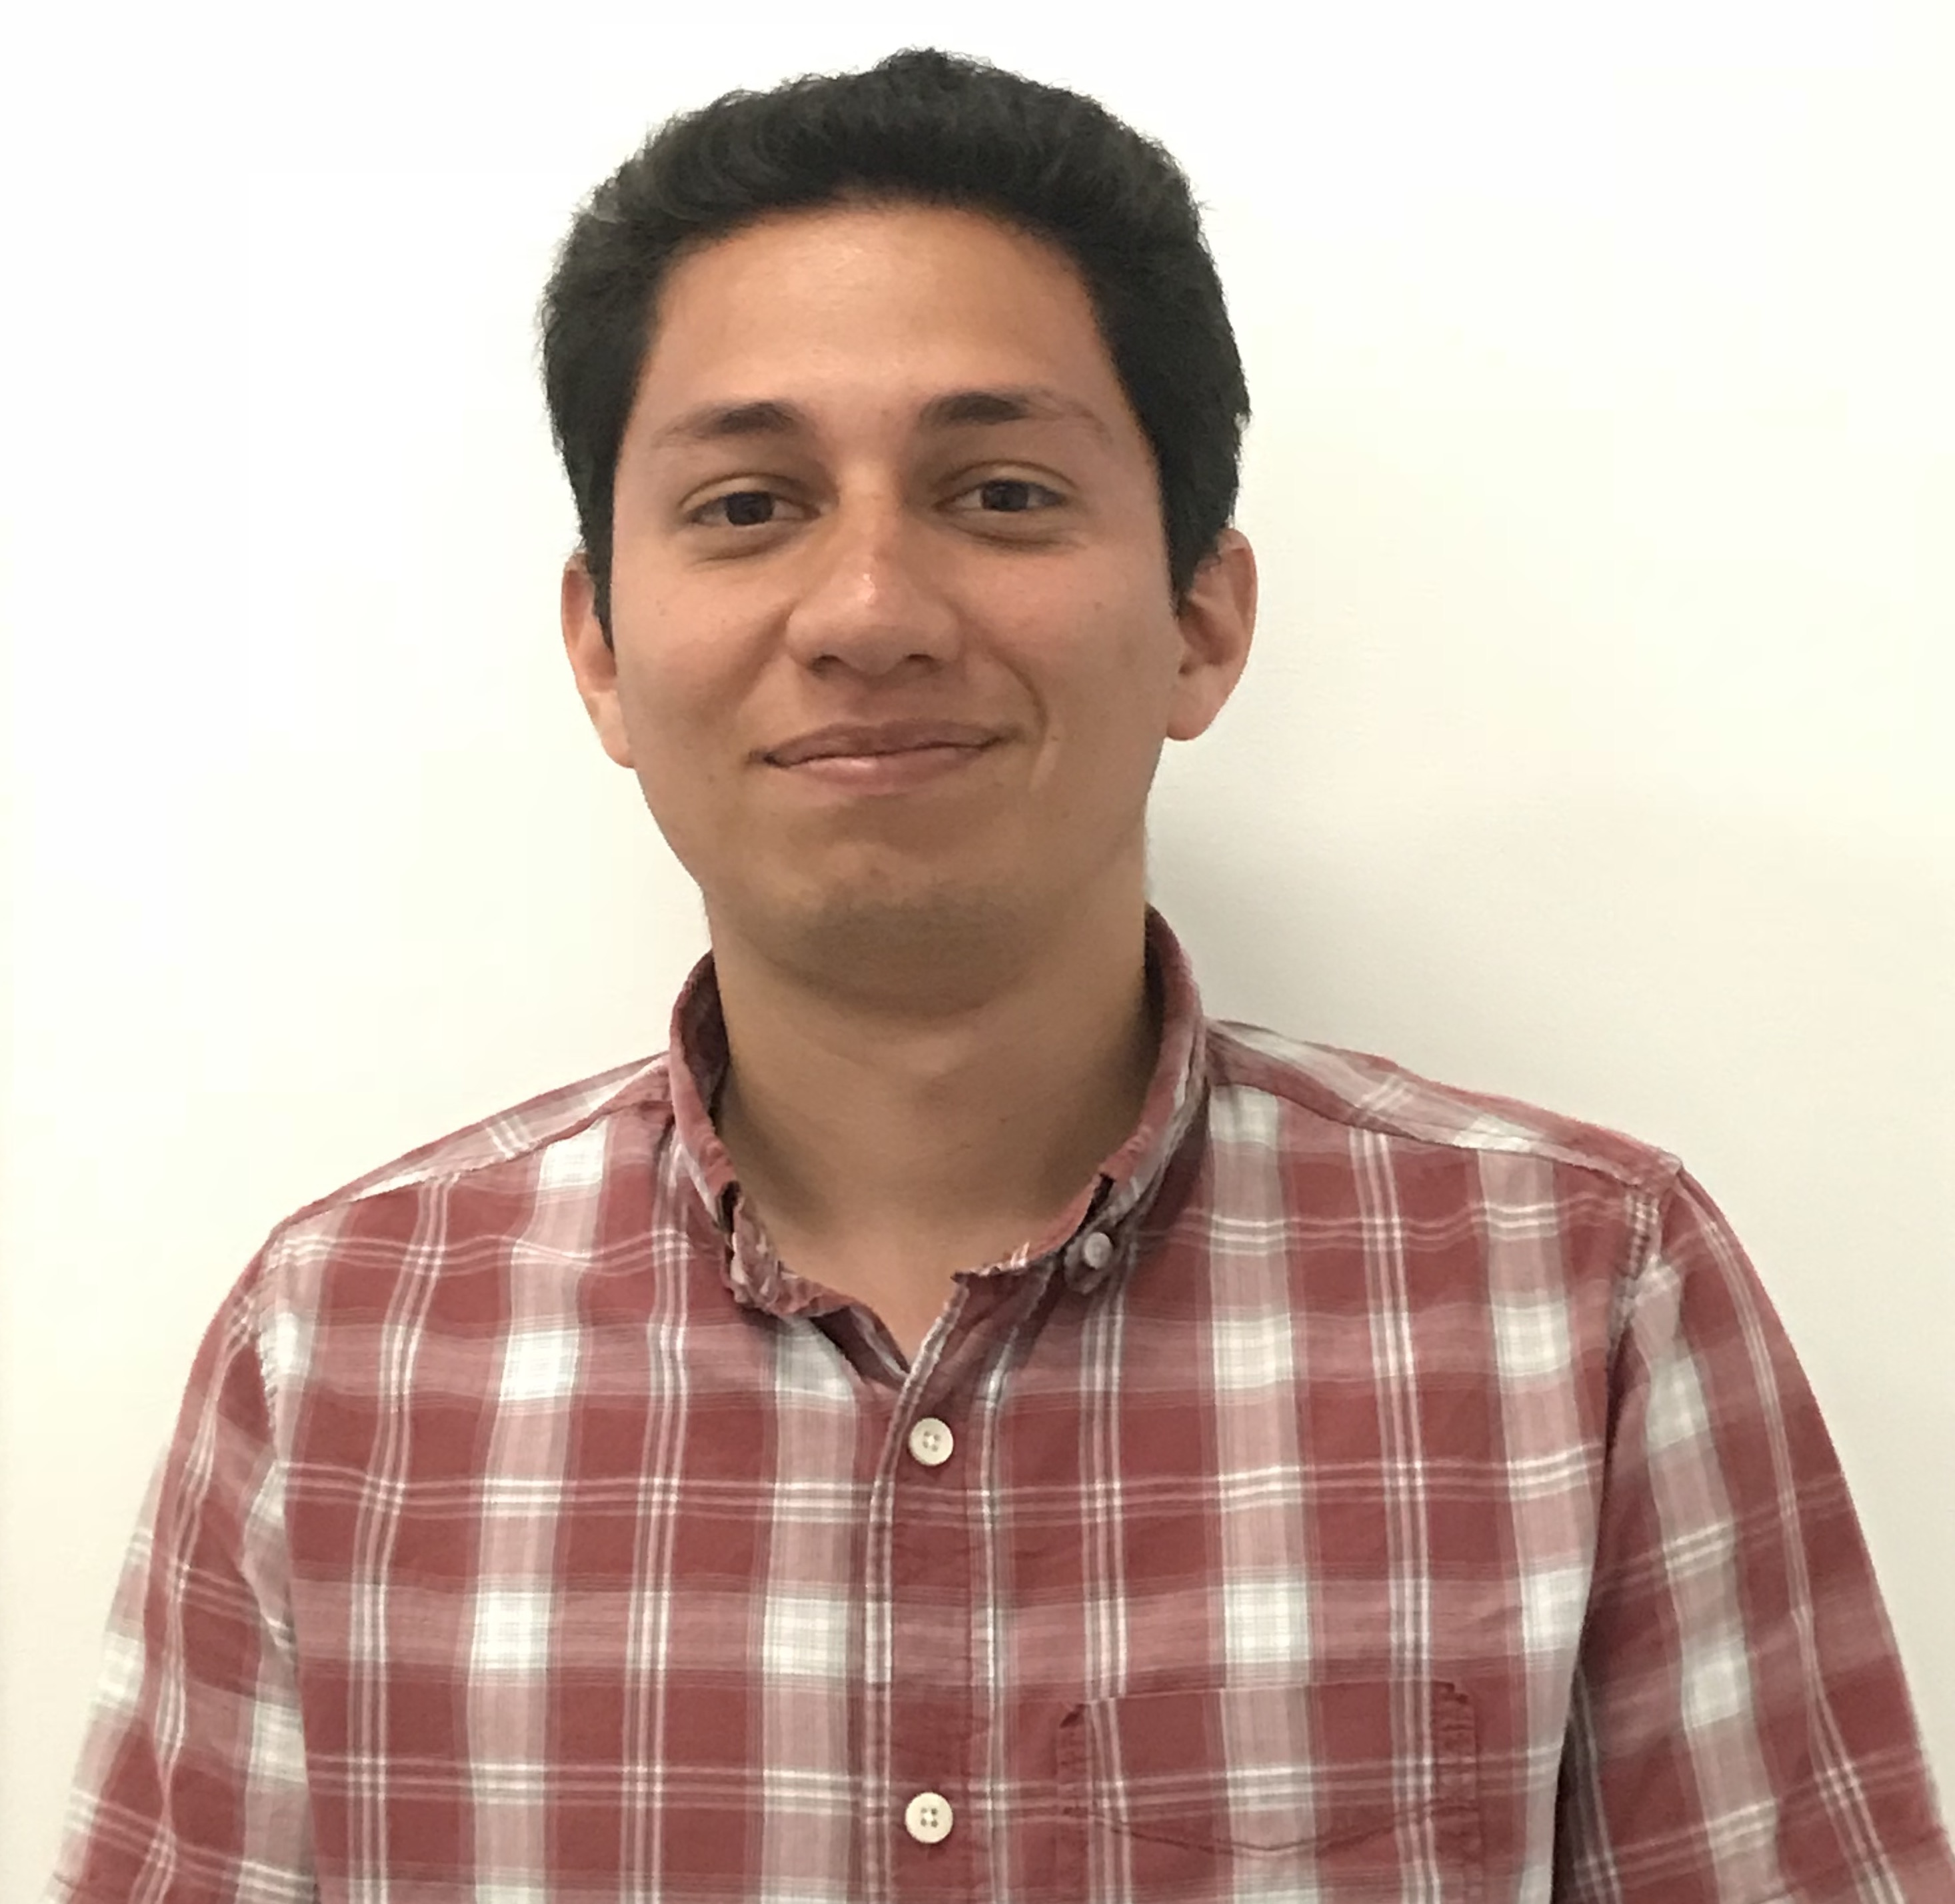
\includegraphics[width=1in,height=1.25in, clip]{BioPhotos/dlr.jpg}}]{David Laredo}
is a graduate student in Mechanical Engineering at UC Merced since 2016. He earned a BS in Computer Science from ESCOM-IPN in 2012 and a Masters in Computer Science from CINVESTAV-IPN in 2015. His research interests are numerical optimization, machine learning for engineering problems, model selection and hyper-parameter tuning.
\end{biography}

\begin{biography}[{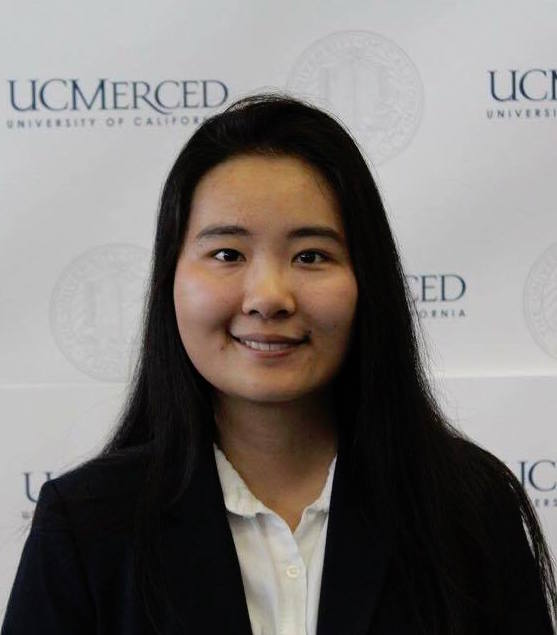
\includegraphics[width=1in,height=1.25in,clip]{BioPhotos/ZhaoyinChen.jpg}}]{Zhaoyin Chen}
is an undergraduate student in Computer Science and Engineering at UC Merced. 
She worked in Applied Controls Lab, where she applied deep learning.
She is interested in database, model training and optimal architecture for engineering problems. She is involved
with the Association for Computing Machinery and serves
on the leadership board as the treasurer. She is a multiple time
recipient of the Chancellor's Honor List award.
\end{biography}

\begin{biography}[{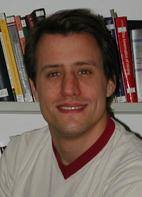
\includegraphics[width=1in,height=1.25in,clip]{BioPhotos/ols.jpg}}]{Oliver Sch\"utze}
received the Diploma degree in mathematics from University
of Bayreuth in 1999, and Ph.D. degree in natural
sciences from University of Paderborn, Germany, in
2004. He is currently a Professor (CINVESTAV-3A Re-searcher) with the Department
of Computer Science, CINVESTAV-IPN, Mexico City, Mexico. He serves as Editor-in-Chief of Mathematical and Computational Applications. His research interests include design and analysis of numerical and evolutionary optimization algorithms.
\end{biography}

\begin{biography}[{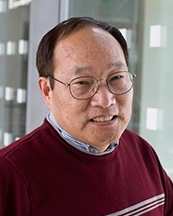
\includegraphics[width=1in,height=1.25in,clip]{BioPhotos/jqs.jpg}}]{Jian-Qiao Sun}
earned a BS in Solid Mechanics from Huazhong University of Science and Technology in 1982, and PhD in Mechanical Engineering from UC Berkeley in 1988.  In 1994, Dr. Sun joined the faculty at University of Delaware until 2007 when he moved to University of California at Merced. He is currently Professor and Chair of Mechanical Engineering. He serves as the Editor-in-Chief of the International Journal of Dynamics and Control.  His research interests include vibrations, controls, energy harvesting, and data-driven modeling and analysis of complex systems.
\end{biography}


